% !TeX program = pdflatex
\documentclass[12pt,a4paper]{article}

\usepackage{avaliacao-template}

% Suporte a acentos dentro dos blocos de código (listings)
\lstset{literate=%
  {á}{{\'a}}1 {à}{{\`a}}1 {â}{{\^a}}1 {ã}{{\~a}}1
  {é}{{\'e}}1 {ê}{{\^e}}1 {í}{{\'i}}1
  {ó}{{\'o}}1 {ô}{{\^o}}1 {õ}{{\~o}}1 {ú}{{\'u}}1
  {ç}{{\c c}}1 {Á}{{\'A}}1 {É}{{\'E}}1 {Ç}{{\c C}}1
}

\renewcommand{\LogoInstituicao}{logo_horizontal_manhuacu.png}
\renewcommand{\NomeAvaliacao}{Avaliação 2 (AV2)}
\renewcommand{\PontuacaoAvaliacao}{2 pontos}
\renewcommand{\CodigoDisciplina}{INF03098}
\renewcommand{\NomeDisciplina}{Engenharia de Software III}
\renewcommand{\DataAvaliacao}{\campo{3.0cm}}
\renewcommand{\ProfessorAvaliacao}{Filipe Fernandes}
\renewcommand{\OrientacoesProva}{%
  \begin{enumerate}[label=\arabic*.]
    \item A prova é individual e sem consulta.
    \item Leia atentamente a contextualização do projeto antes de responder às questões.
    \item Escreva as respostas na folha de respostas, identificando cada arquivo pelo seu caminho completo.
    \item Em arquivos YAML, a indentação faz parte da sintaxe e será considerada na correção.
    \item A interpretação das questões faz parte da avaliação.
  \end{enumerate}
}

\begin{document}

\CapaCadernoQuestoes

\ModoQuestoes
\pagestyle{cadernoQuestoes}
\setcounter{page}{1}
% Contextualização da prova (aparece apenas no caderno de questões)

\section*{Contextualização}

A aplicação \textbf{Copa Resultados} é um webapp que lista todas as partidas da
Copa do Mundo de 2026, da fase de grupos até a final. Os dados são obtidos do
projeto aberto \texttt{openfootball/worldcup.json} e armazenados no banco
\texttt{cupmatches}. A aplicação é composta por três partes:

\begin{itemize}
  \item \textbf{Backend (\texttt{api/})}: API em Node.js, TypeScript, Express e
        Mongoose, com os endpoints \texttt{GET /matches} (retorna o torneio com
        todas as partidas) e \texttt{GET /health} (verificação de saúde). Possui
        script de \emph{seed} que baixa o calendário oficial e popula o banco, e
        testes BDD com Cucumber.
  \item \textbf{Frontend (\texttt{web/})}: aplicação em Vite, TypeScript e React
        que consome a API e exibe as partidas. Em produção, os arquivos estáticos
        são servidos pelo Nginx.
  \item \textbf{Banco de dados}: MongoDB.
\end{itemize}

\begin{figure}[H]
  \centering
  % TODO: substituir o quadro abaixo pelo print do frontend
  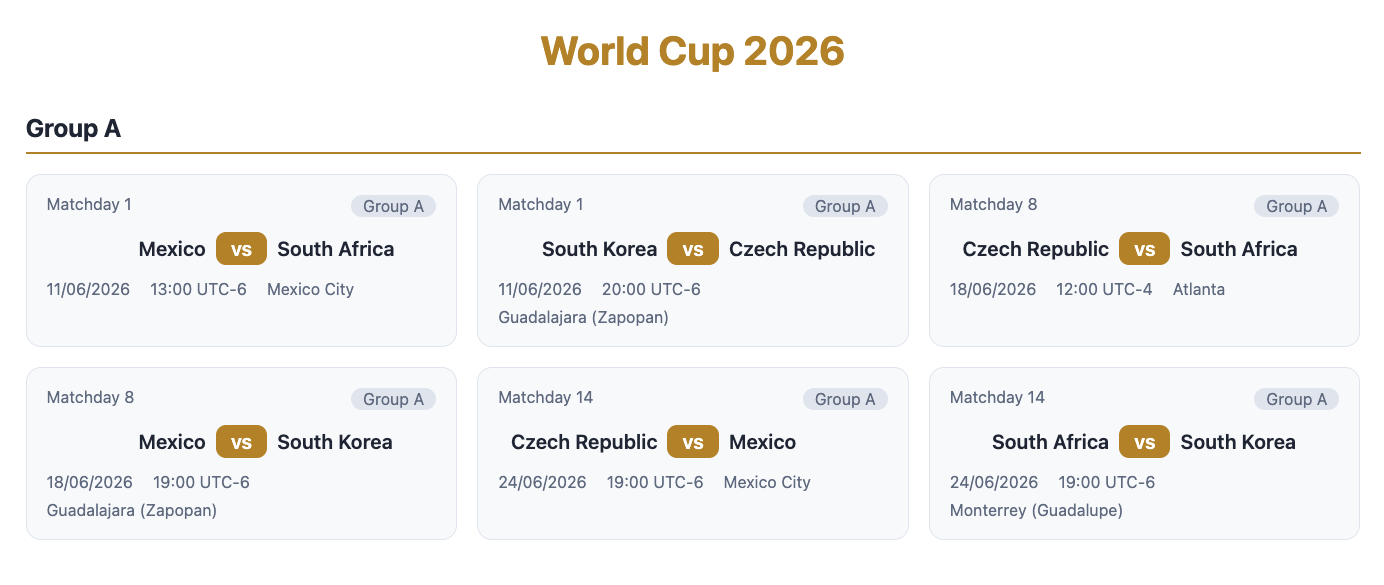
\includegraphics[width=0.9\textwidth]{cupmatches-screenshot.png}
%   \fbox{\parbox[c][6.5cm][c]{0.88\textwidth}{\centering \emph{Espaço reservado
%   para o print da tela principal do frontend}}}
  \caption{Tela principal do webapp Copa Resultados.}
\end{figure}

\subsection*{Estrutura do projeto}

O projeto está pronto e funcional, mas \textbf{ainda não está containerizado}.
A estrutura de pastas é a seguinte (os arquivos marcados são os que você deverá
escrever nesta prova):

\begin{lstlisting}
App/
|-- .github/
|   |-- workflows/
|       |-- api-test-bdd.yml  # <== QUESTAO 3
|-- api/                  # Backend (Node.js + TypeScript + Express + Mongoose)
|   |-- src/              # config/, controllers/, models/, routes/, seed.ts, server.ts
|   |-- features/         # Testes BDD (Cucumber)
|   |-- .env.dev          # Variaveis de ambiente (execucao local)
|   |-- Dockerfile        # <== QUESTAO 1
|-- web/                  # Frontend (Vite + React + TypeScript)
|   |-- src/              # components/, api.ts, App.tsx, main.tsx
|   |-- .env.dev          # Variaveis de ambiente (execucao local)
|   |-- nginx.conf        # Configuracao do Nginx (ja existe, pronta para uso)
|   |-- Dockerfile        # Ja existe, pronto para uso (nao e cobrado)
|-- docker-compose.yml    # <== QUESTAO 2
|-- .env                  # Variável de ambiente (lida automaticamente pelo Docker)
|-- README.md
\end{lstlisting}

\subsection*{Detalhes importantes do projeto}

\begingroup\sloppy
\begin{itemize}
  \item \textbf{Imagens}: Node 20 (\texttt{node:20-alpine}), Nginx
        (\texttt{nginx:alpine}) e MongoDB 7 (\texttt{mongo:7}).
  \item \textbf{Portas internas}: a API escuta na porta \texttt{3000}; o Nginx do
        container web escuta na porta \texttt{80}; o MongoDB usa a porta
        \texttt{27017}.
  \item \textbf{Rede do Docker Compose}: dentro da rede, a API acessa o banco pelo
        \textbf{nome do serviço} (\texttt{mongodb}), e não por \texttt{localhost}.
  \item \textbf{Build do frontend}: a variável \texttt{VITE\_API\_URL} é usada em
        \textbf{tempo de build} do Vite; por isso deve ser passada como
        \emph{build arg} para o Dockerfile do \texttt{web}.
  \item \textbf{Nginx}: o arquivo \texttt{web/nginx.conf} já existe e deve ser
        copiado para \texttt{/etc/nginx/conf.d/\allowbreak default.conf}; o build
        do Vite gera a pasta \texttt{dist}, que deve ser copiada para
        \texttt{/usr/share/\allowbreak nginx/\allowbreak html}.
  \item \textbf{Scripts npm do backend} (\texttt{api/package.json}):
\begin{itemize}
  \item \texttt{npm run dev} --- executa a API em modo de desenvolvimento, com
        recarga automática.
  \item \texttt{npm run build} --- compila o TypeScript para \texttt{dist/}.
  \item \texttt{npm start} --- executa a API já compilada (\texttt{node
        dist/server.js}).
  \item \texttt{npm run seed} --- baixa o calendário oficial e popula o banco.
  \item \texttt{npm run test:bdd} --- executa os testes BDD com Cucumber.
\end{itemize}
  \item \textbf{Variáveis de ambiente da raiz} (usadas pelo Docker Compose), com os
        valores exatos do projeto:

\begin{lstlisting}
API_PORT=3000
WEB_PORT=5173
MONGODB_PORT=27017
MONGODB_DATABASE=cupmatches
MONGODB_URI=mongodb://mongodb:27017/cupmatches
\end{lstlisting}

  \item \textbf{Execução local sem Docker}: os arquivos \texttt{api/.env.dev} e
        \texttt{web/.env.dev} já existem no projeto, com o seguinte conteúdo:

\begin{lstlisting}
# api/.env.dev
PORT=3000
MONGODB_URI=mongodb://localhost:27017/cupmatches

# web/.env.dev
VITE_API_URL=http://localhost:3000
\end{lstlisting}
  \item \textbf{Integração contínua}: o repositório deve possuir o workflow de
        \emph{GitHub Actions} \texttt{.github/\allowbreak workflows/\allowbreak
        api-test-bdd.yml}, que executa os testes BDD da API a cada \emph{push}
        no repositório remoto (detalhado na Questão 3).
  \item \textbf{Frontend já containerizado}: o arquivo \texttt{web/Dockerfile}
        já existe e está pronto para uso; nesta prova você não precisa escrevê-lo.
\end{itemize}
\endgroup

\section*{Questões}
% Questões da AV2 - Containerização e CI da aplicação Copa Resultados
% Os gabaritos das questões são lidos diretamente de Test/snippets/,
% que contém cópias exatas dos arquivos reais do projeto App/.

% 1 - App/api/Dockerfile
\begin{questao}[0,5 ponto]
Escreva o conteúdo completo do arquivo \texttt{App/api/Dockerfile}. O Dockerfile
deve ser \emph{multi-stage}, com duas etapas:

\begin{itemize}
  \item \textbf{\texttt{build}}: instala todas as dependências e compila o
        TypeScript;
  \item \textbf{\texttt{production}}: instala somente as dependências de
        produção e executa a API já compilada.
\end{itemize}

\resposta[22]{Conteúdo exato de \texttt{App/api/Dockerfile}:
\lstinputlisting{snippets/api-Dockerfile.txt}}
\end{questao}

% 2 - App/docker-compose.yml
\begin{questao}[0,5 ponto]
Escreva o conteúdo completo do arquivo \texttt{App/docker-compose.yml},
orquestrando os serviços \texttt{mongodb}, \texttt{api} e \texttt{web}.
Considere que:

\begin{itemize}
  \item as portas expostas no host e as demais configurações devem usar as
        variáveis de ambiente do arquivo \texttt{.env} da raiz
        (apresentadas na contextualização);
  \item os dados do MongoDB devem persistir em um volume nomeado;
  \item o serviço \texttt{api} depende do \texttt{mongodb}, e o serviço
        \texttt{web} depende da \texttt{api};
%   \item o serviço \texttt{web} deve repassar \texttt{VITE\_API\_URL} como
%         \emph{build arg}.
\end{itemize}

\resposta[54]{Conteúdo exato de \texttt{App/docker-compose.yml}:
\lstinputlisting{snippets/docker-compose.txt}}
\end{questao}

% App/.env
% \begin{questao}[0,2 ponto]
% Com base nas variáveis de ambiente apresentadas na contextualização, escreva o
% conteúdo completo do arquivo \texttt{App/.env}, utilizado pelo Docker
% Compose.

% \resposta[10]{Conteúdo exato de \texttt{App/.env}:
% \lstinputlisting{snippets/env-dev.txt}}
% \end{questao}

% 3 - App/.github/workflows/api-test-bdd.yml
\begin{questao}[0,7 ponto]
Escreva o conteúdo completo do arquivo
\texttt{App/.github/workflows/api-test-bdd.yml}, o workflow de
\emph{GitHub Actions} que executa os testes BDD da API a cada \emph{push} no
repositório. Considere que:

\begin{itemize}
  \item o workflow chama-se \texttt{API - Testes BDD} e deve disparar em
        qualquer \emph{push};
  \item há um único \emph{job} chamado \texttt{test-bdd} (nome de exibição
        \texttt{API - testes BDD}) que roda em \texttt{ubuntu-latest};
  \item o \emph{job} usa um \emph{service container} de banco de dados com a
        imagem \texttt{mongo:7}, publicando a porta \texttt{27017:27017};
  \item por padrão, todos os comandos \texttt{run} devem executar no diretório
        \texttt{App/api} (\texttt{working-directory});
  \item o \emph{job} define as variáveis de ambiente
        \texttt{MONGODB\_URI=mongodb://localhost:27017/cupmatches},
        \texttt{PORT=3000} e \texttt{API\_URL=http://localhost:3000};
  \item os passos, nesta ordem, são: 
      \begin{itemize}
            \item \emph{checkout} do código (\texttt{actions/checkout@v4});
            \item configurar o Node.js 20 (\texttt{actions/setup-node@v4});
            \item instalar as dependências;
            \item compilar o TypeScript;
            \item popular o banco com o \emph{seed};
            \item subir a API em segundo plano e aguardar 5 segundos; e
\begin{lstlisting}
run: |
  npm start &
  sleep 5
\end{lstlisting}
            \item executar os testes BDD.
      \end{itemize}
\end{itemize}


% Os \emph{scripts} npm disponíveis são: \texttt{npm install}, \texttt{npm run
% build}, \texttt{npm run seed}, \texttt{npm start} e \texttt{npm run test:bdd}.

\resposta[54]{Conteúdo exato de
\texttt{App/.github/workflows/api-test-bdd.yml}:
\lstinputlisting{snippets/github-actions.txt}}
\end{questao}

% 5 - Sequência de comandos
\begin{questao}[0,3 ponto]
Considere o seguinte cenário: o Docker está iniciado; todos os pacotes do
projeto estão instalados; o link do repositório remoto já foi adicionado ao
projeto; e todas as mudanças estão comitadas. Escreva, na ordem correta, a
sequência de comandos para \textbf{subir os containers} e, em seguida,
\textbf{atualizar o repositório remoto}.

\resposta[10]{Sequência de comandos:
\lstinputlisting{snippets/comandos.txt}
Observação: o \emph{push} dispara automaticamente o workflow
\texttt{api-test-bdd.yml} no GitHub Actions, que executa os testes BDD da API.}
\end{questao}

\label{UltimaPaginaCadernoQuestoes}

\clearpage
\ModoFolhaRespostas
\setcounter{page}{1}
\setcounter{questao}{0}
\IdentificacaoFolhaRespostas
% Questões da AV2 - Containerização e CI da aplicação Copa Resultados
% Os gabaritos das questões são lidos diretamente de Test/snippets/,
% que contém cópias exatas dos arquivos reais do projeto App/.

% 1 - App/api/Dockerfile
\begin{questao}[0,5 ponto]
Escreva o conteúdo completo do arquivo \texttt{App/api/Dockerfile}. O Dockerfile
deve ser \emph{multi-stage}, com duas etapas:

\begin{itemize}
  \item \textbf{\texttt{build}}: instala todas as dependências e compila o
        TypeScript;
  \item \textbf{\texttt{production}}: instala somente as dependências de
        produção e executa a API já compilada.
\end{itemize}

\resposta[22]{Conteúdo exato de \texttt{App/api/Dockerfile}:
\lstinputlisting{snippets/api-Dockerfile.txt}}
\end{questao}

% 2 - App/docker-compose.yml
\begin{questao}[0,5 ponto]
Escreva o conteúdo completo do arquivo \texttt{App/docker-compose.yml},
orquestrando os serviços \texttt{mongodb}, \texttt{api} e \texttt{web}.
Considere que:

\begin{itemize}
  \item as portas expostas no host e as demais configurações devem usar as
        variáveis de ambiente do arquivo \texttt{.env} da raiz
        (apresentadas na contextualização);
  \item os dados do MongoDB devem persistir em um volume nomeado;
  \item o serviço \texttt{api} depende do \texttt{mongodb}, e o serviço
        \texttt{web} depende da \texttt{api};
%   \item o serviço \texttt{web} deve repassar \texttt{VITE\_API\_URL} como
%         \emph{build arg}.
\end{itemize}

\resposta[54]{Conteúdo exato de \texttt{App/docker-compose.yml}:
\lstinputlisting{snippets/docker-compose.txt}}
\end{questao}

% App/.env
% \begin{questao}[0,2 ponto]
% Com base nas variáveis de ambiente apresentadas na contextualização, escreva o
% conteúdo completo do arquivo \texttt{App/.env}, utilizado pelo Docker
% Compose.

% \resposta[10]{Conteúdo exato de \texttt{App/.env}:
% \lstinputlisting{snippets/env-dev.txt}}
% \end{questao}

% 3 - App/.github/workflows/api-test-bdd.yml
\begin{questao}[0,7 ponto]
Escreva o conteúdo completo do arquivo
\texttt{App/.github/workflows/api-test-bdd.yml}, o workflow de
\emph{GitHub Actions} que executa os testes BDD da API a cada \emph{push} no
repositório. Considere que:

\begin{itemize}
  \item o workflow chama-se \texttt{API - Testes BDD} e deve disparar em
        qualquer \emph{push};
  \item há um único \emph{job} chamado \texttt{test-bdd} (nome de exibição
        \texttt{API - testes BDD}) que roda em \texttt{ubuntu-latest};
  \item o \emph{job} usa um \emph{service container} de banco de dados com a
        imagem \texttt{mongo:7}, publicando a porta \texttt{27017:27017};
  \item por padrão, todos os comandos \texttt{run} devem executar no diretório
        \texttt{App/api} (\texttt{working-directory});
  \item o \emph{job} define as variáveis de ambiente
        \texttt{MONGODB\_URI=mongodb://localhost:27017/cupmatches},
        \texttt{PORT=3000} e \texttt{API\_URL=http://localhost:3000};
  \item os passos, nesta ordem, são: 
      \begin{itemize}
            \item \emph{checkout} do código (\texttt{actions/checkout@v4});
            \item configurar o Node.js 20 (\texttt{actions/setup-node@v4});
            \item instalar as dependências;
            \item compilar o TypeScript;
            \item popular o banco com o \emph{seed};
            \item subir a API em segundo plano e aguardar 5 segundos; e
\begin{lstlisting}
run: |
  npm start &
  sleep 5
\end{lstlisting}
            \item executar os testes BDD.
      \end{itemize}
\end{itemize}


% Os \emph{scripts} npm disponíveis são: \texttt{npm install}, \texttt{npm run
% build}, \texttt{npm run seed}, \texttt{npm start} e \texttt{npm run test:bdd}.

\resposta[54]{Conteúdo exato de
\texttt{App/.github/workflows/api-test-bdd.yml}:
\lstinputlisting{snippets/github-actions.txt}}
\end{questao}

% 5 - Sequência de comandos
\begin{questao}[0,3 ponto]
Considere o seguinte cenário: o Docker está iniciado; todos os pacotes do
projeto estão instalados; o link do repositório remoto já foi adicionado ao
projeto; e todas as mudanças estão comitadas. Escreva, na ordem correta, a
sequência de comandos para \textbf{subir os containers} e, em seguida,
\textbf{atualizar o repositório remoto}.

\resposta[10]{Sequência de comandos:
\lstinputlisting{snippets/comandos.txt}
Observação: o \emph{push} dispara automaticamente o workflow
\texttt{api-test-bdd.yml} no GitHub Actions, que executa os testes BDD da API.}
\end{questao}

\label{UltimaPaginaFolhaRespostas}

\end{document}
